\documentclass{tufte-book}
\usepackage[utf8]{inputenc}
\usepackage[english]{babel}
\usepackage{minted}
\usepackage{listings}
\usepackage{mips}
\usepackage{adjustbox}
\usepackage{lstautogobble}
\usepackage{zi4}
\usepackage{eso-pic}
\usepackage[dvipsnames]{xcolor}
\usepackage{graphicx}
\graphicspath{{../images/}}

\usemintedstyle{manni}

% cover photo
\newcommand\BackgroundPic{%
\put(-110,-200){%
\parbox[b][\paperheight]{\paperwidth}{%
\vfill
\centering
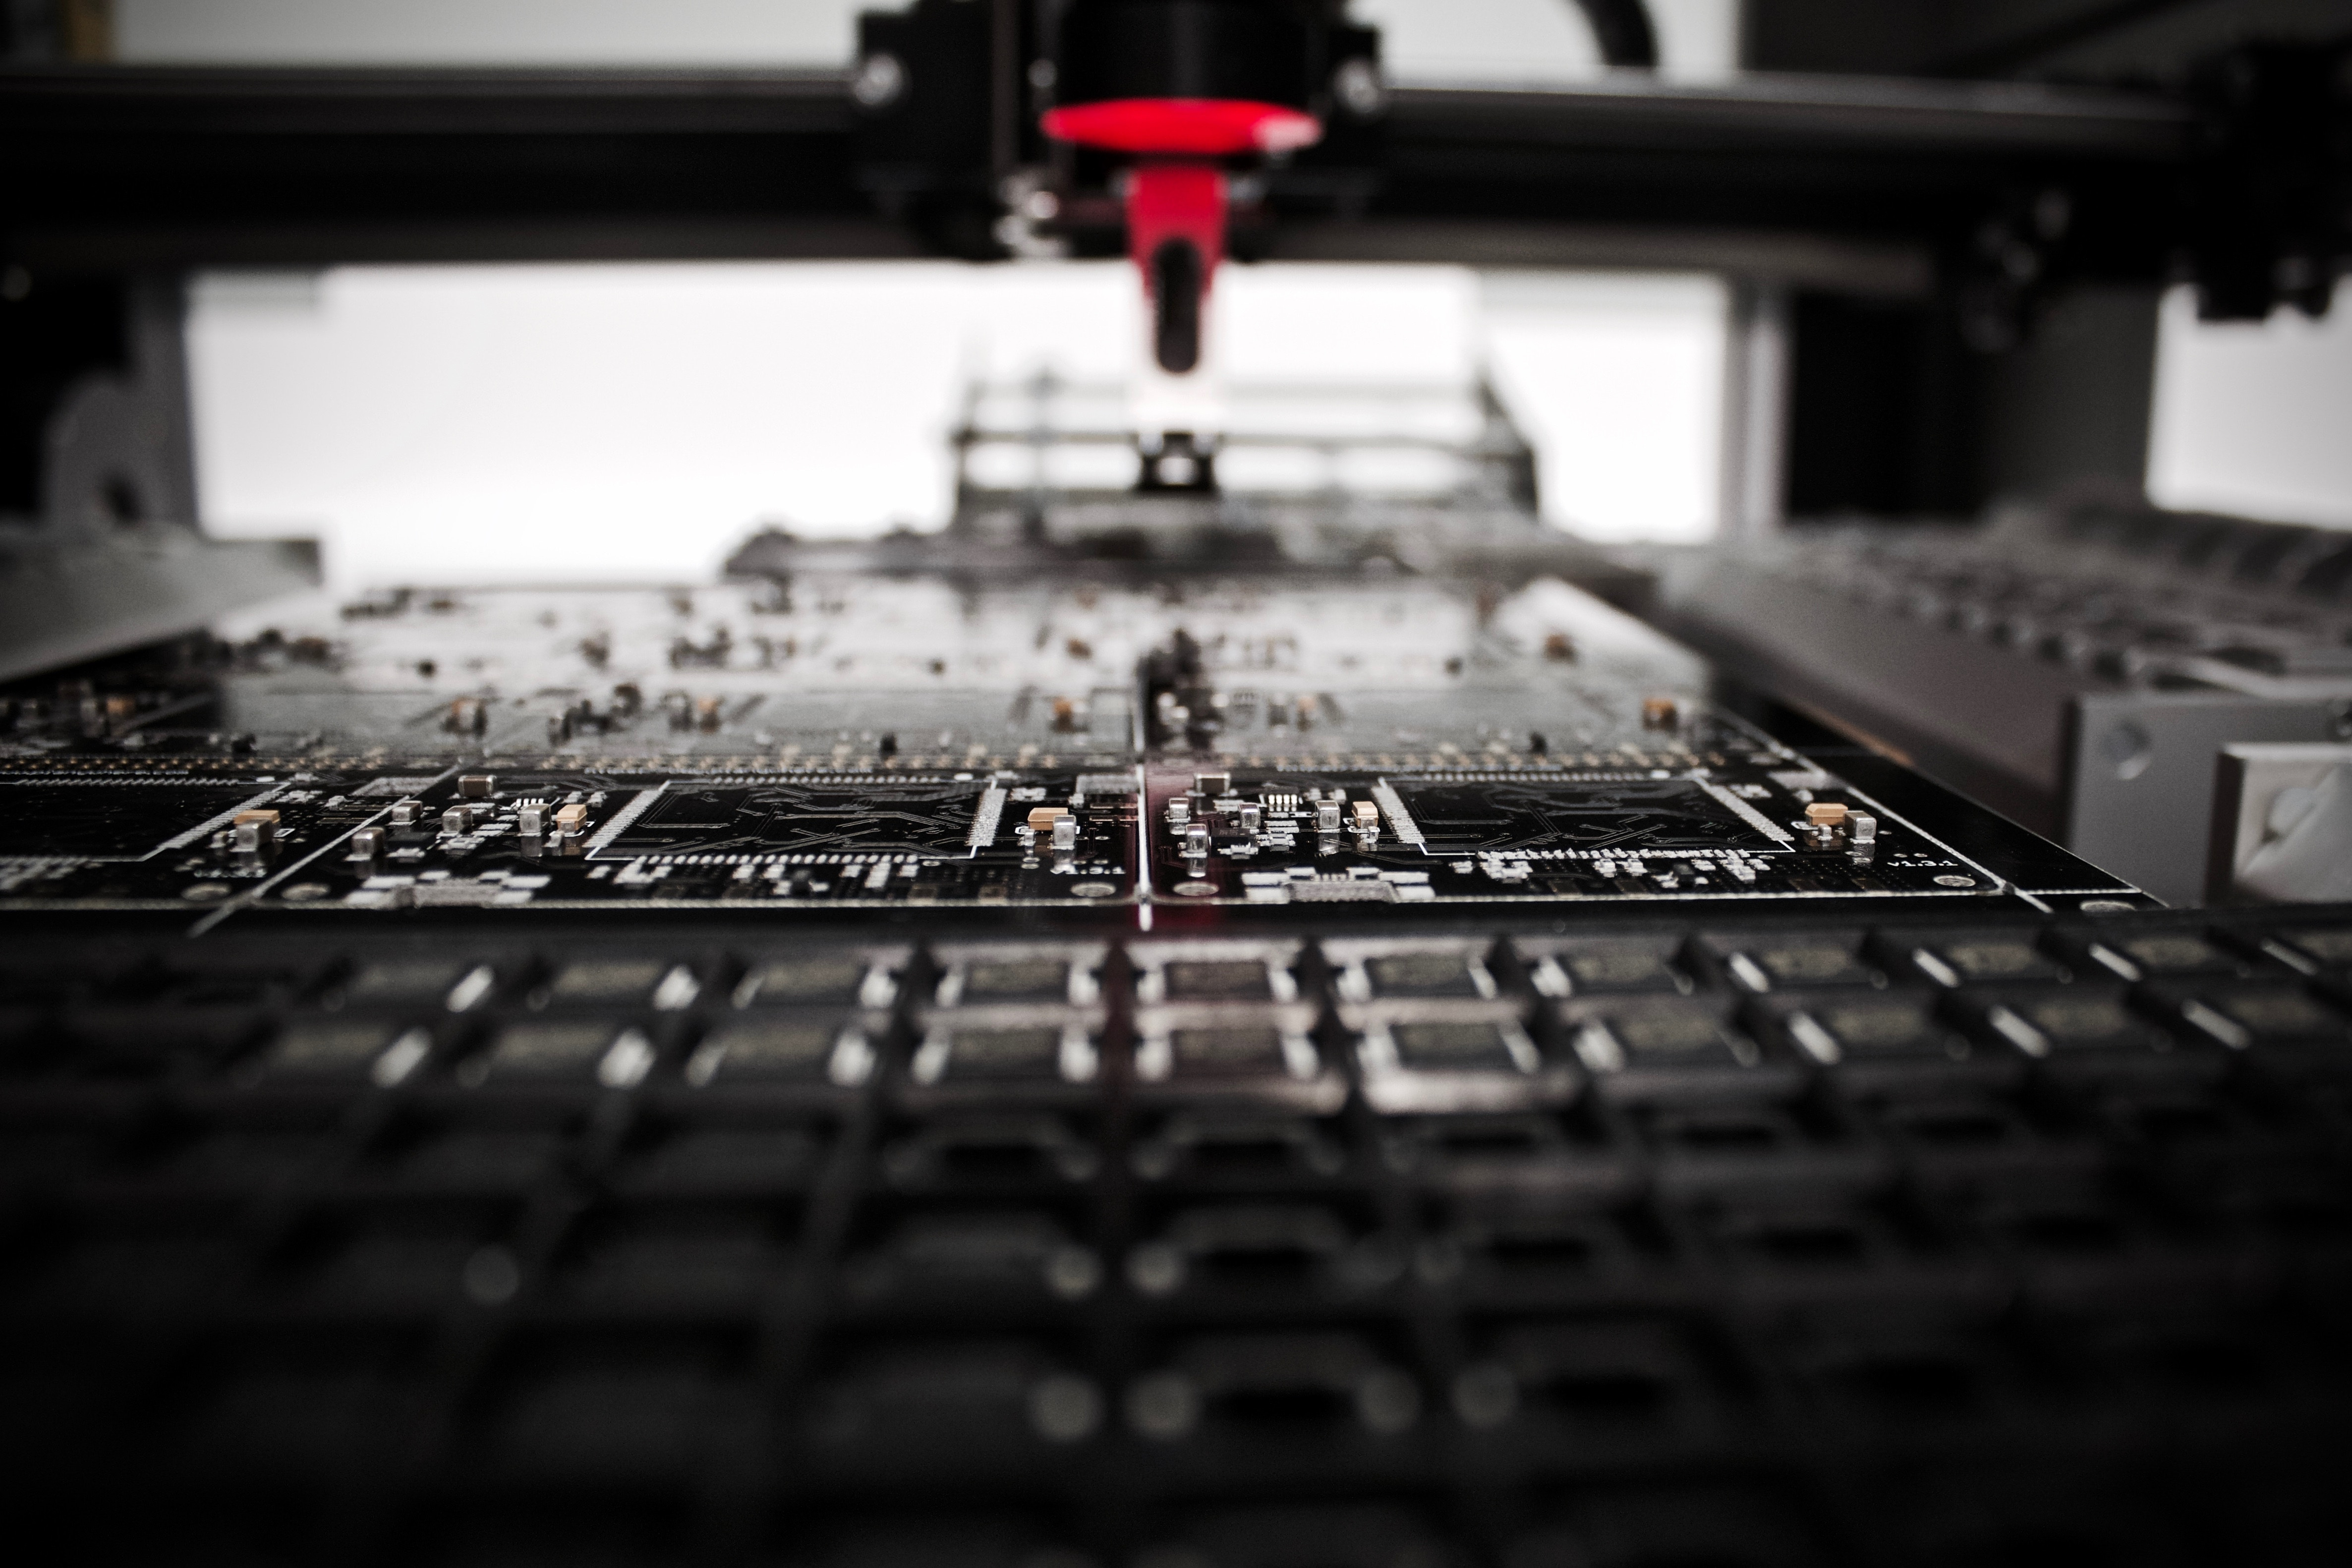
\includegraphics[height=1.3\paperheight,%
keepaspectratio]{assemblycover2}%
\vfill
}}}

\lstset{language=[mips]Assembler}
\lstset{%
  aboveskip=3mm,
  belowskip=3mm,
  showstringspaces=false,
  basicstyle={\ttfamily},
  numbers=none,
  numberstyle=\tiny\color{gray},
  captionpos=none,
  title=\lstname,
  keywordstyle=\bfseries\color{magenta},
  commentstyle=\color{green!50!black},
  stringstyle=\color{red},
  breaklines=true,
  breakatwhitespace=true,
  tabsize=4
}

\setlength{\parindent}{0pt}
\title{Assembly Language}
\author{Richard Robinson}

\begin{document}
\AddToShipoutPicture*{\BackgroundPic}
\frontmatter
\maketitle
\setlength{\parindent}{0pt}
\mainmatter


%%%%%%%%%%%%%%%%%%%%%%%%%%%%%%%%%%%%%%%%%%%%%%%%%%%%%%%%%%%%%%%%%%%%%%
% MAIN DOCUMENT
%%%%%%%%%%%%%%%%%%%%%%%%%%%%%%%%%%%%%%%%%%%%%%%%%%%%%%%%%%%%%%%%%%%%%%

\chapter{Introduction}

\section{Performance Metrics}
There are several metrics of performance of programs by processors. These include
\begin{itemize}
  \item \textit{Execution time}, the total time required for the computer to complete a task (also called response time).
  \item \textit{Bandwidth}, the number of tasks completed per unit time (also called throughput).
  \item \textit{Performance}, the inverse of execution time.
  \item \textit{Clock cycle}, the time for one (processor) clock period, which runs at a constant rate.
\end{itemize}
Consequently, the CPU time is defined as
\marginnote{\textbf{CPI}: the average number of clock cycles per instruction for a program.}
\begin{equation}
  t_{\mathrm{cpu}} = n_{\mathrm{cycles}}/r_{\mathrm{clock}} \quad\mathrm{for}\quad n_{\mathrm{cycles}} = I \times \mathrm{CPI}
\end{equation}
The MIPS unit is another performance metric, given by \begin{equation}
  \textrm{MIPS} = I/t_{\mathrm{exec.}} \cdot 10^6 = r_{\mathrm{clock}} / \mathrm{CPI} \cdot 10^6
\end{equation}

\marginnote{\textbf{MIPS:} A measurement of program execution speed based on the number of millions of instructions.}

\section{RISC-V Syntax}
\textbf{RISC-V} is an assembly language with a basic syntax of
\begin{lstlisting}
  add x1,x2,x3      // x1 = x2 + x3
\end{lstlisting}
The operands \verb|x0-x31| are the 32 registers with \verb|x0| always equaling \verb|0|. Data must be in registers for arithmetic. Additionally, there are $2^{61}$ memory words \verb|Memory[8i]| which may be accessed only by data transfer instructions.

\marginnote{\textbf{Word:} Half of a doubleword; a group of 32 bits.}

\bigskip
In RISC-V, a doubleword is a group of 64 bits. There are never any variables in RISC-V; all variables are converted into respective registers. For example, if \verb|g| and \verb|h| are \verb|x20,x21| and the base address is \verb|x22| of array \verb|A|, then the C code

\marginnote{\textbf{Address}: The index for a data element in a memory array.}

\begin{lstlisting}
  A[z] = h + A[y]
\end{lstlisting}
in RISC-V is translated to
\begin{lstlisting}
  ld  x9,8y(x22)     // temp reg x9 gets A[y]
  add x9,x21,x9      // temp reg x9 gets h + A[y]
  sd  x9,8z(x22)     // stores x9 into A[z]
\end{lstlisting}
The reg added to form the address (\verb|x22|) is the \textit{base reg} and the DTI constant (64) is the \textit{offset}. To get the proper byte address, the offset to be added to the base reg is $8c$ where $c$ is the initial constant.

\marginnote{\textbf{Byte}: A group of 8 bits; there are 8 bytes in a doubleword.}

\bigskip
This implies that the byte address of an element is a multiple of 8; that is, element $i$ has byte address $8i$ where the first element is $i_0$.

\section{Binary \& Hexadecimal}
Binary to decimal base is calculated via \begin{equation}
  \sum x_i 2^i
\end{equation}
where $x_i$ is the $i$th digit starting at $i=0$ and increasing leftwards. In RISC-V, the least or most sig. bit is the rightmost or leftmost bit, respectively.

\bigskip
Two's complement representation for signed binary numbers assigns leading 0s as positive and leading 1s as negative. The complements are related by \begin{equation}
  \overline{x} + 1 = -x
\end{equation}
Binary is used in the instruction format, which represents an instruction in 6 fields, typically the \textit{R}-type:
\begin{enumerate}
  \item \verb|opcode|: basic op of the instruction (7b).
  \item \verb|rd|: reg dest operand; gets result of op (5b).
  \item \verb|funct3/7|: additional opcodes (3/7b).
  \item \verb|rs2/1|: second / first reg source operand (5b).
\end{enumerate}

In Hexadecimal, all groups of 4 binary digits may be represented by a single hexadecimal digit, ranging from $0 - 9, a - f$ such that \begin{center}
  \verb|9 = 1001| \qquad \verb|a = 1010| \qquad \verb|f = 1111|
\end{center}

\section{Logical \& Conditional Ops}
The typical logical operators occur in RISC-V, as do:
\begin{enumerate}
  \item Shift left / right (\verb|sll| / \verb|srl|): moves all bits in a doubleword left / right, filling emptied bits with 0s. Shifting left $i$ bits is equal to multiplying by $2^i$.
  \item Bitwise XOR (\verb|xor|): an operation which returns 1 only if the values differe in the two operands.
  \item Bitwise NOT (\verb|xori|): inverts the bits in a doubleword; equivalent to XOR with one operand being \verb|11...1|.
\end{enumerate}
For conditional statements, the commands \verb|bne| and \verb|beq| are used. For example,
\begin{verbatim}
  if (i == j) f = g + h; else f = g - h
\end{verbatim}
in C where \verb|f-g| are \verb|x19-x23|, the equivalent RISC-V code is
\begin{lstlisting}
        bne x22, x23, Else    // goto Else if i~=j
        add x19, x20, x21     // f=g+h if i == j
        beq x0,   x0, Exit    // goto Exit
  Else: sub x19, x20, x21     // f=g-h if i~=j
  Exit:
\end{lstlisting}
Likewise, for loops, the same commands are used in addition to the label \verb|Loop:|. For example,
\begin{verbatim}
  while (save[i] == k) i++
\end{verbatim}
in C where \verb|i,k,save| are \verb|x22,x24,x25|, the code is
\begin{lstlisting}
  Loop: sll x10, x22, 3     // treg x10=8i
        add x10, x10, x25   // x10 = save[i]
        ld x9, 0(x10)       // treg x9 = save[i]
        bne x9. x24, Exit   // goto Exit if
                            // save[i]~=k
        add x22, x22, 1     // i++
        beq x0, x0, Loop    // goto Loop
  Exit:
\end{lstlisting}
This can be extended to the comparison \verb|0 <= x < y|, which is valid for the index out-of-bounds check. For example, the check \verb$x20 >=$ \verb$x11 || x20 < 0$ is given by \verb$bgey x20, x11, OutOfBounds$.

\chapter{RISC-V Operation}


\end{document}
